\section{Objectives}

\begin{frame}
	\frametitle{\secname}
	\begin{columns}
		\begin{column}{0.38\textwidth}
			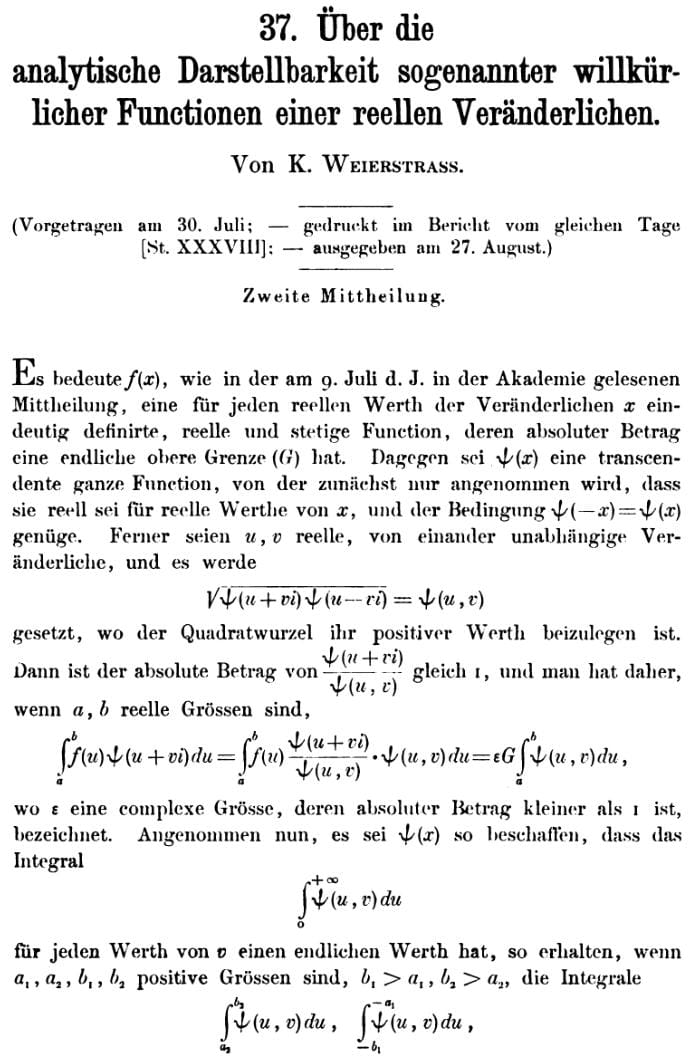
\includegraphics[width=0.3\paperwidth]{original_approximation}
		\end{column}
		\begin{column}{0.58\textwidth}
			\begin{itemize}
				\item

				      Weierstraß proved the \alert{approximation theorem} at
				      the age of 70.
				      He used the
				      \alert{Weierstraß transform}~\cite{weierstrass1885,Schep2007}.

				      \fcolorbox{DarkBlue}{yellow}{
					      \begin{math}
						      \displaystyle
						      \forall f\in C\left(\mathds{R},\mathds{R}\right):
						      F\left(\theta\right)=
						      \frac{1}{\sqrt{4\pi}}
						      \int\limits_{-\infty}^{\infty}
						      f\left(y\right)
						      \exp\left(
						      -\frac{\left(\theta-y\right)^{2}}{4}
						      \right)\dl y.
					      \end{math}
				      }

				\item

				      In 1912, Bernstein made a direct proof with the
				      \alert{Bernstein polynomial}~\cite{Saha2021}.

				\item

				      Proof the \alert{Fejér's theorem}~\cite{Fejér1903}.

				\item

				      Proof the \alert{Stone – Weierstraß theorem} in the
				      real, complex, quaternion and locally compact versions.

				\item

				      Proof the \alert{Bishop's theorem}~\cite{Rudin1991}.
			\end{itemize}
		\end{column}
	\end{columns}

	\note{
		A little of story, Weierstraß was interested in the heat
		equation, he develop la Weierstraß transform.

		\

		.
	}
\end{frame}